\begin{apendicesenv}

\partapendices

\chapter{Apêndice 1 - Protótipos}

Este apêndice apresenta os protótipos do jogo feitos no figma. Ele complementa as informações discutidas no trabalho, fornecendo detalhes adicionais sobre a etapa de idealização do produto final.

Figura~\ref{fig:prototipo-menu} Protótipo menu inicial

\begin{figure}[htbp]
    \centering
    \caption{Menu inicial}
    \label{fig:prototipo-menu}
    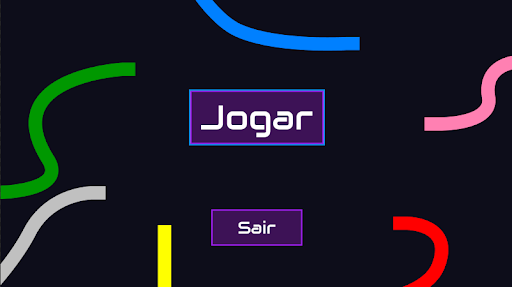
\includegraphics[width=0.7\textwidth]{figuras/prototipo-menu.png}
    \legend{Fonte: Elaboração própria}
\end{figure}

Figura~\ref{fig:prototipo-lobby} Protótipo Seleção dos jogadores - Sala do jogo

\begin{figure}[htbp]
    \centering
    \caption{Sala de iniciação}
    \label{fig:prototipo-lobby}
    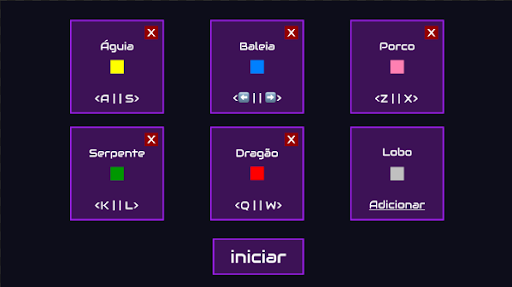
\includegraphics[width=0.7\textwidth]{figuras/prototipo-lobby.png}
    \legend{Fonte: Elaboração própria}
\end{figure}

Figura~\ref{fig:prototipo-in-game} Protótipo Cena do Jogo

\begin{figure}[htbp]
    \centering
    \caption{Tela do jogo}
    \label{fig:prototipo-in-game}
    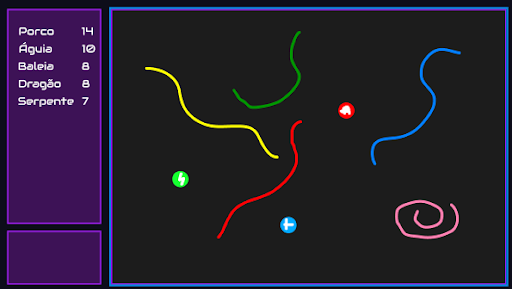
\includegraphics[width=0.7\textwidth]{figuras/prototipo-in-game.png}
    \legend{Fonte: Elaboração própria}
\end{figure}

Figura~\ref{fig:prototipo-end-game} Protótipo Fim do Jogo

\begin{figure}[htbp]
    \centering
    \caption{Fim do jogo - tela de vitória}
    \label{fig:prototipo-end-game}
    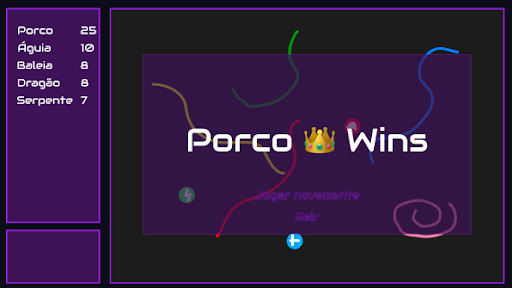
\includegraphics[width=0.7\textwidth]{figuras/prototipo-end-game.png}
    \legend{Fonte: Elaboração própria}
\end{figure}

section{Menu inicial}

\chapter{Apêndice 2 - Imagem dos poderes com ìcones}

Durante a prototipação a idealização dos poderes foi feita de forma que tente representar bem seus feitos. A Figura~\ref{fig:prototipo-poderes} tem o protótipo dos poderes e suas habilidades.

\begin{figure}[htbp]
    \centering
    \caption{Ícones dos poderes}
    \label{fig:prototipo-poderes}
    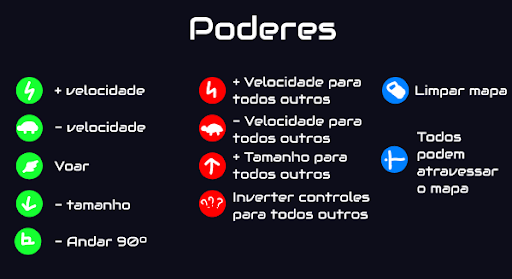
\includegraphics[width=0.7\textwidth]{figuras/prototipo-poderes.png}
    \legend{Fonte: Elaboração própria}
\end{figure}

\chapter{Apêndice 3 - Tarefas do Trello}

Figura~\ref{fig:trello-tarefas}, quadro do trello que foi utilizado para guiar as tarefas ao longo das semanas.

\begin{figure}[htbp]
    \centering
    \caption{Lista de tarefas}
    \label{fig:trello-tarefas}
    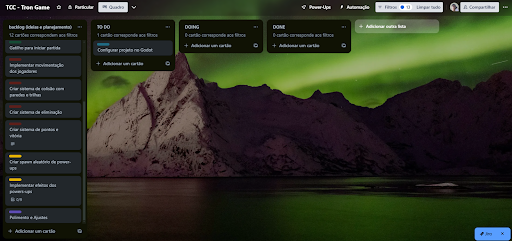
\includegraphics[width=0.7\textwidth]{figuras/trello-quadro.png}
    \legend{Fonte: Elaboração própria}
\end{figure}


\end{apendicesenv}
